\documentclass{article}
\usepackage{graphicx} % Required for inserting images
\usepackage[greek]{babel}
\selectlanguage{greek}

\title{Τεχνικές Βελτιστοποίησης - Εργασία 1}
\author{Ρουσομάνης Γεώργιος (ΑΕΜ: 10703)}
\date{Νοέμβριος 2024}

\begin{document}

\maketitle

\section*{Εισαγωγή}

Σκοπός της συγκεκριμένης εργασίας είναι η ελαχιστοποίηση ορισμένων κυρτών συναρτήσεων 
σε ένα προκαθορισμένο διάστημα $[\alpha, \beta]$. Για τον σκοπό αυτό θα χρησιμοποιηθούν 
οι μέθοδοι Διχοτόμου, Χρυσού Τομέα, $Fibonacci$ και Διχοτόμου με χρήση παραγώγου. Για κάθε 
μέθοδο θα γίνει μία σύντομη περιγραφή του τρόπου λειτουργίας της ενώ θα παρατεθούν τα 
πλεονεκτήματα και τα μειονεκτήματά της κάθε μίας. Στην συνέχεια θα γίνει ερμηνεία και αξιολόγηση 
των αποτελεσμάτων που λαμβάνουμε αντιπαραβάλλοντάς τα με όσα γνωρίζουμε από την θεωρία. 
Τέλος θα γίνει ένας συγκριτικός σχολιασμός πάνω στην αποδοτικότητα των μεθόδων για τις 
υπό μελέτη συναρτήσεις.

\section*{Θέμα 1}
\textbf{Μέθοδος Διχοτόμου}

Ξεκινώντας από ένα αρχικό διάστημα $[\alpha, \beta]$, στο οποίο γνωρίζουμε ότι υπάρχει 
το ελάχιστο, υπολογίζουμε δύο σημεία εντός του διαστήματος και συμμετρικά ως προς το 
κέντρο του $x_1=\frac{\alpha + \beta}{2} - \epsilon, x_2=\frac{\alpha + \beta}{2} + \epsilon$, 
όπου $\epsilon$ μία μικρή τιμή. Υπολογίζουμε τις τιμές της συνάρτησης $f(x_1)$ και $f(x_2)$. 
Εάν $f(x_1) < f(x_2)$, τότε το ελάχιστο βρίσκεται στο διάστημα $[\alpha, x_2]$. 
Διαφορετικά το ελάχιστο βρίσκεται στο $[x_1, \beta]$. Επαναλαμβάνουμε τη διαδικασία 
στο νέο διάστημα αναζήτησης, μέχρι το διάστημα να είναι αρκετά μικρό, 
σύμφωνα με ένα προκαθορισμένο όριο ανοχής $l$. Τα πλεονέκτημα αυτής της μεθόδου είναι η απλότητά
της και το ότι δεν απαιτεί την γνώση της παραγώγου της υπό μελέτη συνάρτησης. 
Τα μειονεκτήματά της είναι ότι συγκλίνει αργά στο επιθυμητό διάστημα ενώ απαιτείται ο υπολογισμός 
της αντικειμενικής συνάρτησης δύο φορές σε κάθε επανάληψη αυξάνοντας το υπολογιστικό κόστος.

Στο Σχήμα~\ref{fig:task1_plot1} βλέπουμε τον αριθμό των υπολογισμών της αντικειμενικής συνάρτησης
συναρτήσει της απόστασης $\epsilon$ από την διχοτόμο για σταθερό τελικό εύρος 
αναζήτησης $l = 0.01$. Παρατηρούμε ότι ο αριθμός των υπολογισμών, άρα και των επαναλήψεων, αυξάνεται
με την αύξηση της απόστασης από την διχοτόμο. Μάλιστα η αύξηση αυτή γίνεται εντονότερη όταν το
$\epsilon$ τείνει στο $\frac{l}{2}$. Αυτό μπορεί εύκολα να ερμηνευτεί καθώς σε κάθε
επανάληψη $k$ το διάστημα αναζήτησης γίνεται $[\alpha_k, \frac{\alpha_k + \beta_k}{2} + \epsilon]$ 
αν $f(x_{2k}) > f(x_{1k})$ και $[\frac{\alpha_k + \beta_k}{2} - \epsilon, \beta_k]$ διαφορετικά. Επομένως, με την
αύξηση του $\epsilon$ περιορίζεται λιγότερο το διάστημα αναζήτησης απαιτώντας μεγαλύτερο αριθμό επαναλήψεων
για να επιτευχθεί η επιθυμητή ακρίβεια. Επίσης παρατηρούμε ότι οι γραφικές παραστάσεις ταυτίζονται για
τις τρεις συναρτήσεις. Ο αριθμός των υπολογισμών της αντικειμενικής συνάρτησης δίνεται από την σχέση
\[ n = \left\lceil 2 log_2\left(\frac{\beta - \alpha}{l}\right) \right\rceil \]
και εξαρτάται από το αρχικό εύρος αναζήτησης και το διάστημα ανοχής $l$ και όχι από τις ιδιαιτερότητες
της κυματομορφής.

\begin{figure}
    \centering
    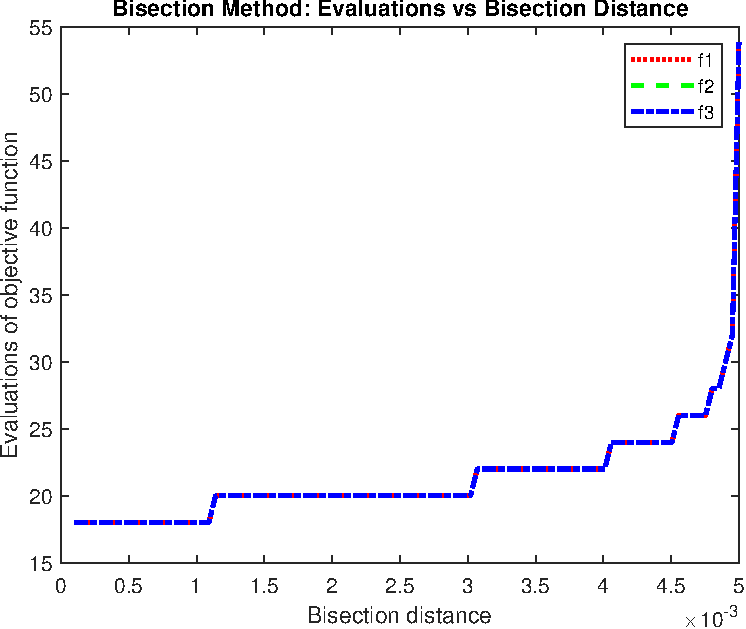
\includegraphics[width=0.75\linewidth]{plots/task1_plot1.pdf}
    \caption{Αριθμός υπολογισμών της αντικειμενικής συνάρτησης στη μεθόδου διχοτόμου συναρτήσει της απόστασης $\epsilon$ για $l=0.01$}
    \label{fig:task1_plot1}
\end{figure}

Παρόμοια συμπεράσματα προκύπτουν κρατώντας σταθερό το $\epsilon = 0.001$ και μεταβάλλοντας το $l$.
Στο Σχήμα~\ref{fig:task1_plot2}, καθώς αυξάνεται το $l$ το πλήθος των υπολογισμών μειώνεται καθώς 
υπάρχει μεγαλύτερη ανοχή στο τελικό αποτέλεσμα. Οι γραφικές παραστάσεις και πάλι ταυτίζονται 
για τον λόγο που αναφέρθηκε παραπάνω.

\begin{figure}
    \centering
    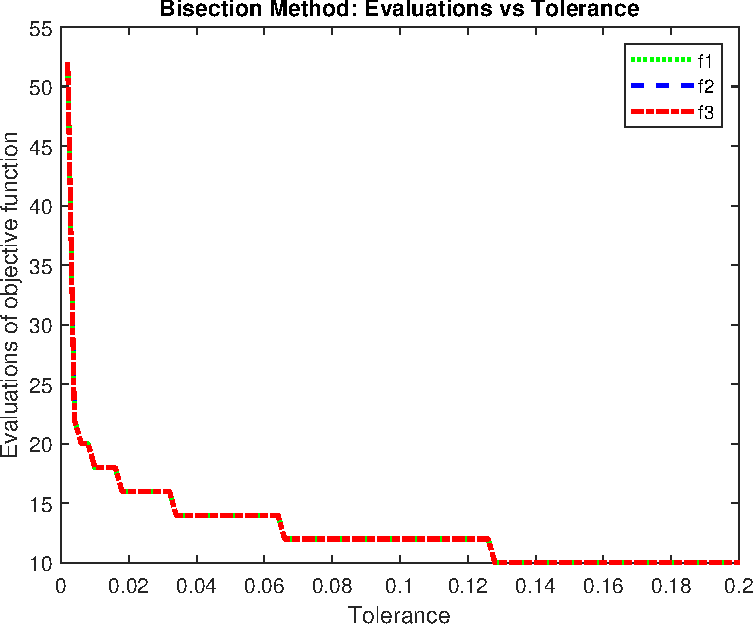
\includegraphics[width=0.75\linewidth]{plots/task1_plot2.pdf}
    \caption{Αριθμός υπολογισμών της αντικειμενικής συνάρτησης για τη μεθόδου της διχοτόμου συναρτήσει του διαστήματος $l$ για $\epsilon = 0.001$}
    \label{fig:task1_plot2}
\end{figure}

Στο Σχήμα~\ref{fig:task1_plot3} βλέπουμε την μεταβολή του διαστήματος αναζήτησης $[\alpha_k, \beta_k]$ 
σε κάθε επανάληψη για διάφορες τιμές του $l$. Παρατηρούμε ότι για $l = 0.14$ απαιτούνται πέντε
επαναλήψεις σε κάθε συνάρτηση, για $l = 0.04$ επτά επαναλήψεις και για $l = 0.002$ δεκαέξι επαναλήψεις.

\begin{figure}
    \centering
    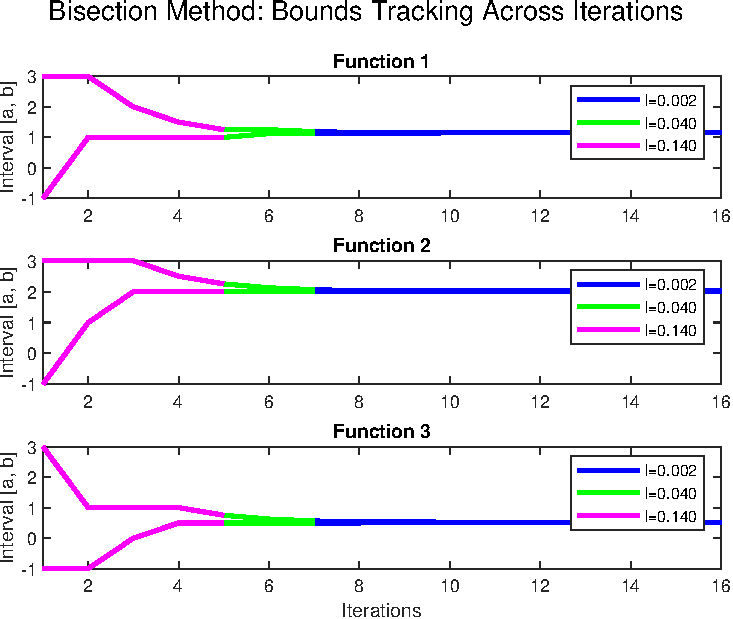
\includegraphics[width=0.75\linewidth]{plots/task1_plot3.pdf}
    \caption{Μεταβολή του διαστήματος $[\alpha_k, \beta_k]$ σε κάθε επανάληψη της μεθόδου διχοτόμησης για διάφορες τιμές του $l$}
    \label{fig:task1_plot3}
\end{figure}

\section*{Θέμα 2}
\textbf{Μέθοδος του Χρυσού Τομέα}

Η διαφορά της μεθόδου του Χρυσού Τομέα ως προς την μέθοδο της διχοτόμησης έγγυται στην επιλογή των 
ενδιάμεσων σημείων. Έστω ότι στην $k$ επανάληψη το διάστημα αναζήτησης είναι το $[\alpha_k, \beta_k]$. 
Τα ενδιάμεσα σημεία $x_{1k}, x_{2k}$ είναι αναλογικά κατανεμημένα στο $[\alpha_k, \beta_k]$ 
σύμφωνα με την αναλογία του χρυσού τομέα
\[ x_{1k} = \alpha_k + \frac{\beta_k - \alpha_k}{\phi} \]
\[ x_{2k} = \beta_k - \frac{\beta_k - \alpha_k}{\phi} \]
όπου $\phi=(1 + \sqrt{5}) / 2$ ο λόγος της χρυσής τομής. 
Έπειτα κάνουμε τα εξής:
\begin{itemize}
    \item Αν $f(x_{1k}) \geq f(x_{2k})$ τότε το ελάχιστο βρίσκεται στο $[x_{1k}, \beta_k]$. 
    Θέτουμε λοιπόν $\alpha_{k+1} = x_{1k}$, $\beta_{k+1} = \beta_k$.
    Προσαρμόζουμε τα ενδιάμεσα σημεία $x_{2k+1}, x_{1k+1}$ ώστε να είναι αναλογικά 
    κατανεμημένα στο νέο διάστημα $[\alpha_{k+1}, \beta_{k+1}]$, δηλαδή έχουμε
    $x_{2k+1} = \alpha_{k+1} + (\beta_{k+1} - \alpha_{k+1})/\phi$,
    $x_{1k+1} = x_{2k}$
    και υπολογίζουμε την $f(x_{2k+1})$.
    \item Αν $f(x_{1k}) < f(x_{2k})$ τότε το ελάχιστο βρίσκεται στο $[\alpha_k, x_{2k}]$.
    Θέτουμε λοιπόν $\alpha_{k+1} = \alpha_k, \beta_{k+1} = x_{2k}$.
    Προσαρμόζουμε τα ενδιάμεσα σημεία $x_{2k+1}, x_{1k+1}$ ώστε να είναι αναλογικά 
    κατανεμημένα στο νέο διάστημα $[\alpha_{k+1}, \beta_{k+1}]$, δηλαδή έχουμε
    $x_{2k+1} = x_{1k}$,
    $x_{1k+1} = \beta_{k+1} - (\beta_{k+1} - \alpha_{k+1})/\phi$
    και υπολογίζουμε την $f(x_{1k+1})$.
\end{itemize}
Ο αλγόριθμος τερματίζει μόλις ικανοποιηθεί η απαίτηση για μία προκαθορισμένη ακρίβεια $l < \beta_k - \alpha_k$.

Το πλεονέκτημα της συγκεκριμένης μεθόδου είναι η απαίτηση μόνο ενός επιπλέον
υπολογισμού της αντικειμενικής συνάρτησης είτε στο $x_{2k+1}$ είτε στο $x_{1k+1}$
σε κάθε επανάληψη, έχοντας μικρότερο υπολογιστικό κόστος από την μέθοδο της διχοτόμου.
Επίσης δεν απαιτεί την γνώση της παραγώγου της αντικειμενικής συνάρτησης.

Από το Σχήμα~\ref{fig:task1_plot2} και Σχήμα~\ref{fig:task2_plot1} βλέπουμε ότι για το ίδιο
εύρος τιμών του $l$ η μέθοδος του Χρυσού Τομέα απαιτεί σημαντικά μικρότερο αριθμό υπολογισμών
της αντικειμενικής συνάρτησης $f$. Επίσης, και σε αυτή την περίπτωση οι γραφικές παραστάσεις
και των τριών συναρτήσεων ταυτίζονται. Το πλήθος των υπολογισμών δίνεται
από την σχέση
\[ n =\left\lceil \frac{ln\left(\frac{\beta_1 - \alpha_1}{l}\right)}{ln\phi} \right\rceil + 1 \]
όπου $\phi = 1.618$ ο λόγος της χρυσής τομής. Επομένως, ο αριθμός των επαναλήψεων που απαιτούνται 
για να επιτευχθεί μία συγκεκριμένη ανοχή εξαρτάται μόνο από το αρχικό μήκος του διαστήματος και την 
ανοχή που έχουμε θέσει, και όχι από τη μορφή της κάθε συνάρτησης.

\begin{figure}
    \centering
    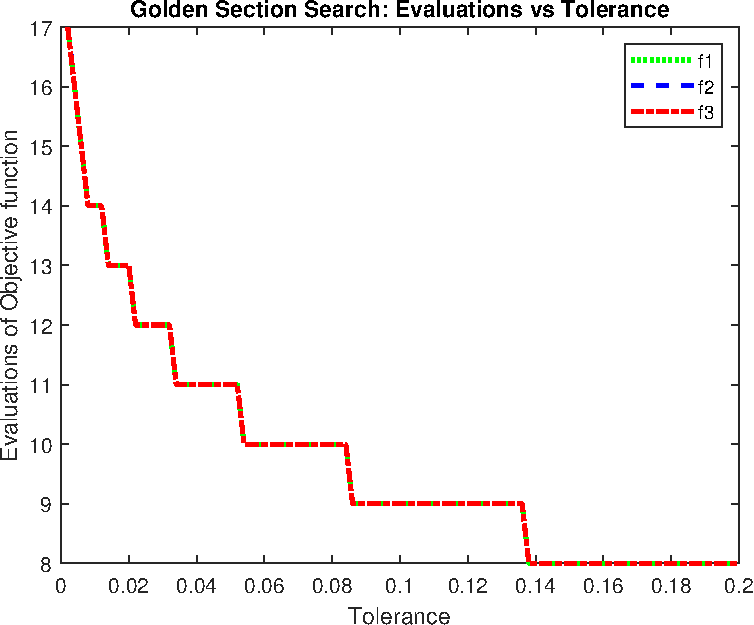
\includegraphics[width=0.75\linewidth]{plots/task2_plot1.pdf}
    \caption{Αριθμός υπολογισμών της αντικειμενικής συνάρτησης για την μεθόδου του χρυσού τομέα συναρτήσει του διαστήματος $l$}
    \label{fig:task2_plot1}
\end{figure}

Στο Σχήμα~\ref{fig:task2_plot2} βλέπουμε την μεταβολή του διαστήματος $[\alpha_k, \beta_k]$ 
σε κάθε επανάληψη για διάφορες τιμές του $l$. Παρατηρούμε ότι για $l = 0.14$ απαιτούνται επτά
επαναλήψεις, για $l = 0.04$ δέκα επαναλήψεις και για $l = 0.002$ δεκαέξι επαναλήψεις. Επομένως
για τις περιπτώσεις των $l = 0.14$ και $l = 0.04$ η μέθοδος του χρυσού τομέα εκτέλεσε περισσότερες
επαναλήψεις από αυτή της διχοτόμου ώστε να επιτύχει την επιθυμητή ακρίβεια, ωστόσο το υπολογιστικό
κόστος της μεθόδου του χρυσού τομέα παραμένει μικρότερο. Ακόμα για μεγάλες ακρίβειες επιτυγχάνει
τον ίδιο αριθμό επαναλήψεων με την μέθοδο διχοτόμησης αλλά με λιγότερους υπολογισμούς.

\begin{figure}
    \centering
    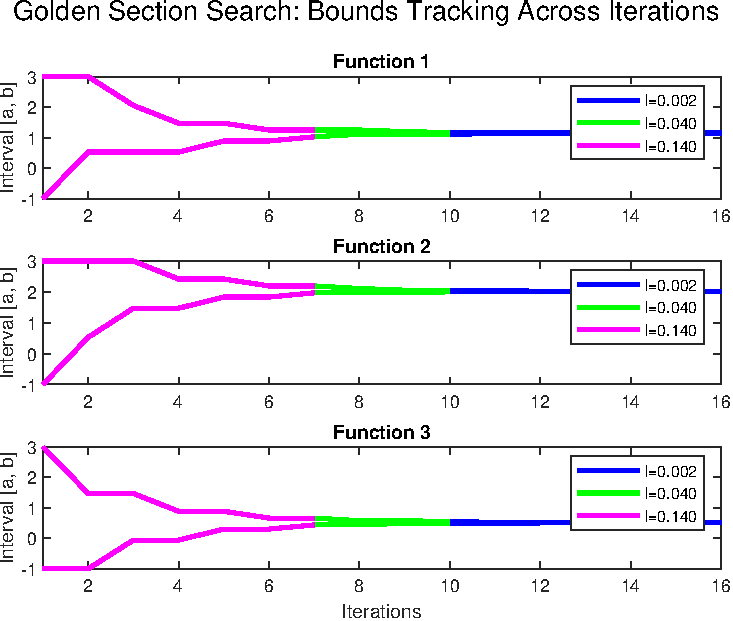
\includegraphics[width=0.75\linewidth]{plots/task2_plot2.pdf}
    \caption{Μεταβολή του διαστήματος $[\alpha_k, \beta_k]$ σε κάθε επανάληψη της μεθόδου του χρυσού τομέα για διάφορες τιμές του $l$}
    \label{fig:task2_plot2}
\end{figure}

\section*{Θέμα 3}
\textbf{Μέθοδος $Fibonacci$}

Η μέθοδος $Fibonacci$ διαφοροποιείται από αυτή του χρυσού τομέα στο ότι το υποδιάστημα αναζήτησης στην $k$
επανάληψη δεν συνδέεται με αυτό της $k - 1$ επανάληψης με μία σταθερά, αλλά μεταβάλλεται από επανάληψη σε
επανάληψη. Επίσης, απαιτεί τον εκ των προτέρων προσδιορισμό των συνολικών υπολογισμών $n$ της αντικειμενικής
συνάρτησης έτσι ώστε $F_n > \frac{\beta_1 - \alpha_1}{l}$. Πιο συγκεκριμένα, έστω ότι στην $k$ επανάληψη το 
διάστημα αναζήτησης είναι $[\alpha_k, \beta_k]$. Τα εσωτερικά σημεία $x_{1k}, x_{2k}$ επιλέγονται έτσι ώστε 
να είναι αναλογικά κατανεμημένα στο $[\alpha_k, \beta_k]$ με βάση τους διαδοχικούς όρους 
$F_{n-k-1}, F_{n-k}, F_{n-k+1}$ της ακολουθίας $Fibonacci$
\[ x_{1k} = \alpha_k + \frac{F_{n-k-1}}{F_{n-k+1}}(\beta_k - \alpha_k) \] 
\[ x_{2k} = \alpha_k + \frac{F_{n-k}}{F_{n-k+1}}(\beta_k - \alpha_k). \]
Έπειτα, επαναλαμβάνουμε τα εξής:
\begin{itemize}
    \item Αν $f(x_{1k}) > f(x_{2k})$, τότε το ελάχιστο θα βρίσκεται στο διάστημα $[x_{1k}, \beta_k]$.
    Θέτουμε λοιπόν $a_{k+1} = x_{1k}$ και $b_{k+1} = b_k$. Προσαρμόζουμε τα εσωτερικά σημεία έτσι ώστε
    να είναι αναλογικά κατανεμημένα στο $[\alpha_{k+1}, \beta_{k+1}]$ με βάση την ακολουθία $Fibonacci$,
    δηλαδή $x_{1k+1} = x_{2k}$ και $x_{2k+1} = \alpha_{k+1} + \frac{F_{n-k-1}}{F_{n-k}}(\beta_{k+1} - \alpha_{k+1})$
    και υπολογίζουμε την $f(x_{2k+1})$.
    \item Αν $f(x_{1k}) < f(x_{2k})$, τότε το ελάχιστο θα βρίσκεται στο διάστημα $[\alpha_k, x_{2k}]$.
    Θέτουμε λοιπόν $\alpha_k = \alpha_{k+1}$ και $b_{k+1} = x_{2k}$. Προσαρμόζουμε τα εσωτερικά σημεία έτσι ώστε
    να είναι αναλογικά κατανεμημένα στο $[\alpha_{k+1}, \beta_{k+1}]$ με βάση την ακολουθία $Fibonacci$,
    δηλαδή $x_{2k+1} = x_{1k}$ και $x_{1k+1} = \alpha_{k+1} + \frac{F_{n-k-2}}{F_{n-k}}(\beta_{k+1} - \alpha_{k+1})$
    και υπολογίζουμε την $f(x_{1k+1})$.
\end{itemize}
Ο αλγόριθμος τερματίζει όταν $k = n - 2$. Τότε θέτουμε $x_{1n} = x_{1n-1}$ και $x_{2n} = x_{1n-1} + \epsilon$, όπου
$\epsilon > 0$ μία σταθερά. Αν $f(x_{1n}) > f(x_{2n})$ το σημείο ελαχίστου θα ανήκει στο $[x_{1n}, \beta_{n-1}]$.
Διαφορετικά θα ανήκει στο $[\alpha_{n-1}, x_{2n}]$.

Το πλεονέκτημα αυτής της μεθόδου, όπως και αυτής του χρυσού τομέα, είναι η απαίτηση μόνο ενός επιπλέον
υπολογισμού της αντικειμενικής συνάρτησης σε κάθε επανάληψη. Ωστόσο η μέθοδος $fibonacci$ είναι πιο αποδοτική
από αυτή του χρυσού τομέα καθώς συγκλίνει γρηγορότερα στο επιθυμητό διάστημα. Το μειονέκτημά της είναι η
απαίτηση για τον εκ των προτέρων υπολογισμό των συνολικών επαναλήψεων καθώς και ο υπολογισμός όρων της ακολουθίας
$fibonacci$.

Στο Σχήμα~\ref{fig:task3_plot1} φαίνεται ο αριθμός των υπολογισμών της αντικειμενικής συνάρτησης συναρτήσει
του τελικού διαστήματος αναζήτησης $l$. Προφανώς όσο μειώνεται το $l$ απαιτείται μεγαλύτερος αριθμός 
επαναλήψεων κάτι το οποίο φαίνεται και από την σχέση $F_n > (\beta_1 - \alpha_1) / l$. Συνεπώς,
ο αριθμός των επαναλήψεων δεν εξαρτάται από τα ιδιαίτερα χαρακτηριστικά της εκάστοτε συνάρτησης παρά
μόνο από το αρχικό διάστημα αναζήτησης και το τελικό εύρος, εξού και η ταύτιση των τριών γραφικών παραστάσεων.
Επίσης, από το Σχήμα~\ref{fig:task2_plot1} και Σχήμα~\ref{fig:task3_plot1} παρατηρούμε ότι η μέθοδος $fibonacci$
απαιτεί μικρότερο ή ίσο αριθμό υπολογισμών της αντικειμενικής συνάρτησης από την μέθοδο του χρυσού τομέα, κάτι το οποίο
συμφωνεί με τα όσα γνωρίζουμε από την θεωρία.

\begin{figure}
    \centering
    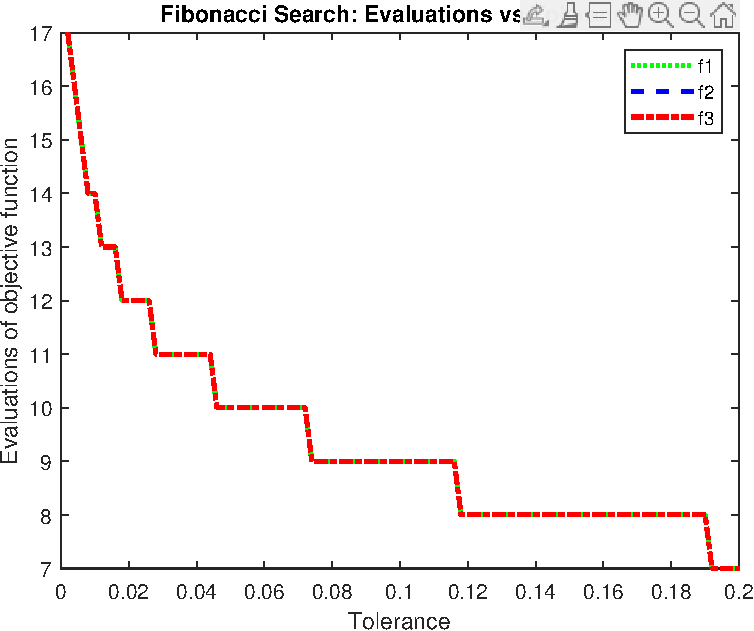
\includegraphics[width=0.75\linewidth]{plots/task3_plot1.pdf}
    \caption{Αριθμός υπολογισμών της αντικειμενικής συνάρτησης για τη μέθοδο $fibonacci$ συναρτήσει του διαστήματος $l$}
    \label{fig:task3_plot1}
\end{figure}

Στο Σχήμα~\ref{fig:task3_plot2} φαίνεται η μεταβολή του διαστήματος αναζήτησης σε κάθε επανάληψη για διάφορες τιμές
του $l$. Παρατηρούμε ότι για τις συγκεκριμένες τιμές του $l$, η μέθοδος $fibonacci$ απαιτεί το ίδιο πλήθος 
επαναλήψεων με την μέθοδο του χρυσού τομέα.

\begin{figure}
    \centering
    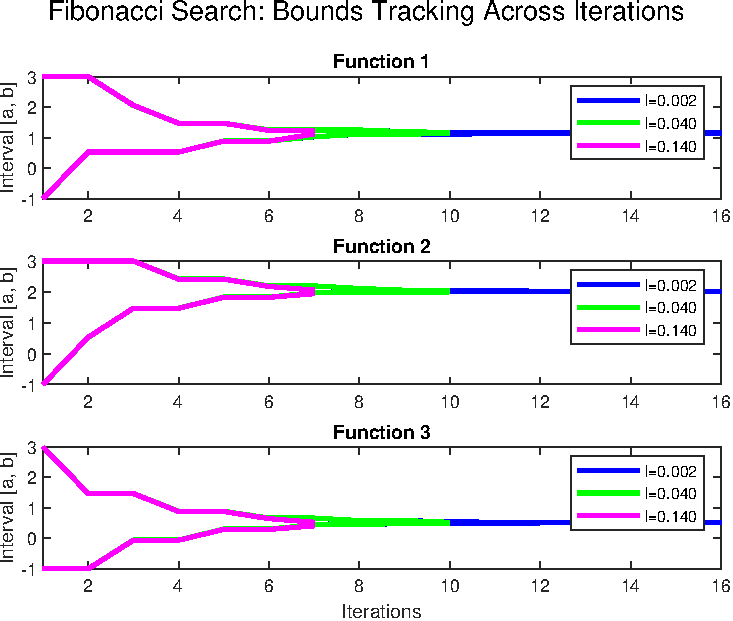
\includegraphics[width=0.75\linewidth]{plots/task3_plot2.pdf}
    \caption{Μεταβολή του διαστήματος $[\alpha_k, \beta_k]$ σε κάθε επανάληψη της μεθόδου $fibonacci$ για διάφορες τιμές του $l$}
    \label{fig:task3_plot2}
\end{figure}

\section*{Θέμα 4}
\textbf{Μέθοδος διχοτόμου με χρήση παραγώγου}

Η συγκεκριμένη μέθοδος απαιτεί, όπως και η μέθοδος $fibonacci$, τον εκ των προτέρων υπολογισμό του συνολικού αριθμού
$n$ των επαναλήψεων ώστε να ικανοποιείται η σχέση $\left(\frac{1}{2}\right)^{n} \leq \frac{l}{\beta_1 - \alpha_1}$.
Έστω $[\alpha_k, \beta_k]$ το διάστημα αναζήτησης στην $k$ επανάληψη. Θέτουμε $x_k = \frac{\beta_k + \alpha_k}{2}$
και υπολογίζουμε $\frac{df(x)}{dx}\Big|_{x = x_k}$. Αν $\frac{df(x)}{dx}\Big|_{x = x_k} = 0$ το $x_k$ είναι το
ελάχιστο σημείο και ο αλγόριθμος τερματίζει. Διαφορετικά, αν $\frac{df(x)}{dx}\Big|_{x = x_k} > 0$, το ελάχιστο
θα βρίσκεται στο διάστημα $[\alpha_{k}, x_k]$ οπότε θέτουμε $\alpha_{k+1} = \alpha_k$ και $\beta_{k+1} = x_k$. 
Τέλος, αν $\frac{df(x)}{dx}\Big|_{x = x_k} < 0$ το ελάχιστο θα βρίσκεται στο διάστημα $[x_k, \beta_k]$ οπότε 
θέτουμε $a_{k+1} = x_k$ και $\beta_{k+1} = \beta_k$. Ο αλγόριθμος τερματίζει αν $k = n$.

Το πλεονέκτημα της μεθόδου είναι η ταχύτερη σύγκλιση έναντι των άλλων τριών μεθόδων λόγω της χρήσης παραγώγου.
Επίσης δεν απαιτεί η αντικειμενική συνάρτηση να είναι κυρτή για τον εντοπισμό του ελαχίστου ενώ ο υπολογισμός
της παραγώγου γίνεται μία φορά σε κάθε επανάληψη. Το μειονέκτημα της είναι ότι απαιτεί την γνώση της παραγώγου 
της αντικειμενικής συνάρτησης καθώς και τον εκ των προτέρων υπολογισμό του αριθμού των επαναλήψεων.

Στο Σχήμα~\ref{fig:task4_plot1} φαίνεται ο αριθμός των υπολογισμών της παραγώγου συναρτήσει του τελικού εύρους $l$.
Όπως και στις προηγούμενες μεθόδους οι γραφικές παραστάσεις των τριών αντικειμενικών συναρήσεων ταυτίζονται
καθώς ο αριθμός των επαναλήψεων εξαρτάται μόνο από το αρχικό διάστημα αναζήτησης και το εύρος $l$ κάτι το οποίο
διαπιστώνουμε και από την σχέση $\left(\frac{1}{2}\right)^{n} \leq \frac{l}{\beta_1 - \alpha_1}$.

\begin{figure}
    \centering
    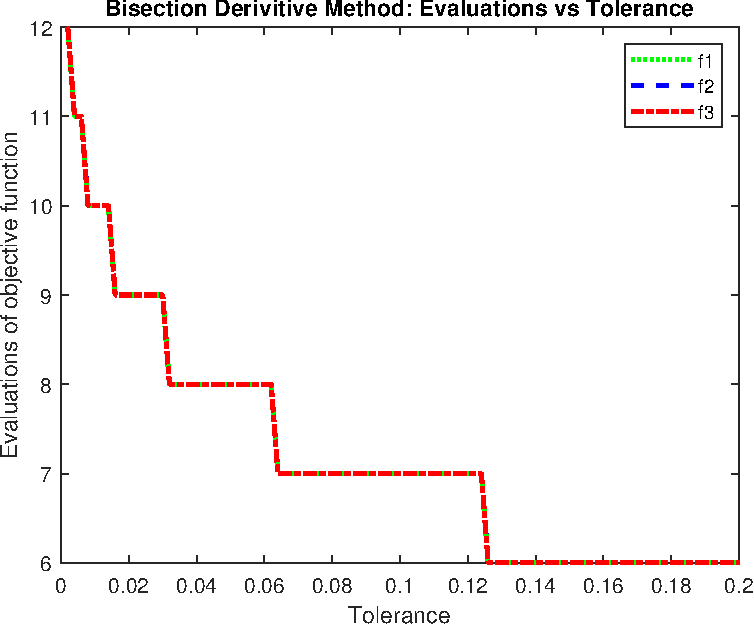
\includegraphics[width=0.75\linewidth]{plots/task4_plot1.pdf}
    \caption{Αριθμός υπολογισμών της παραγώγου της αντικειμενικής συνάρτησης για την μέθοδο της διχοτόμου με χρήση παραγώγου συναρτήσει του εύρους $l$}
    \label{fig:task4_plot1}
\end{figure}

Στο Σχήμα~\ref{fig:task4_plot2} φαίνεται η μεταβολή του διαστήματος αναζήτησης σε κάθε επανάληψη για διάφορες τιμές
του $l$. Παρατηρούμε ότι για $l = 0.14$ απαιτούνται πέντε επαναλήψεις, για $l = 0.04$ επτά επαναλήψεις και για 
$l = 0.002$ έντεκα επαναλήψεις. Συνεπώς η μέθοδος διχοτόμου με χρήση παραγώγου συγκλίνει ταχύτερα από τις τρεις
άλλες μεθόδους για όλες τις τιμές του $l$, όπως άλλωστε αναμέναμε.

\begin{figure}
    \centering
    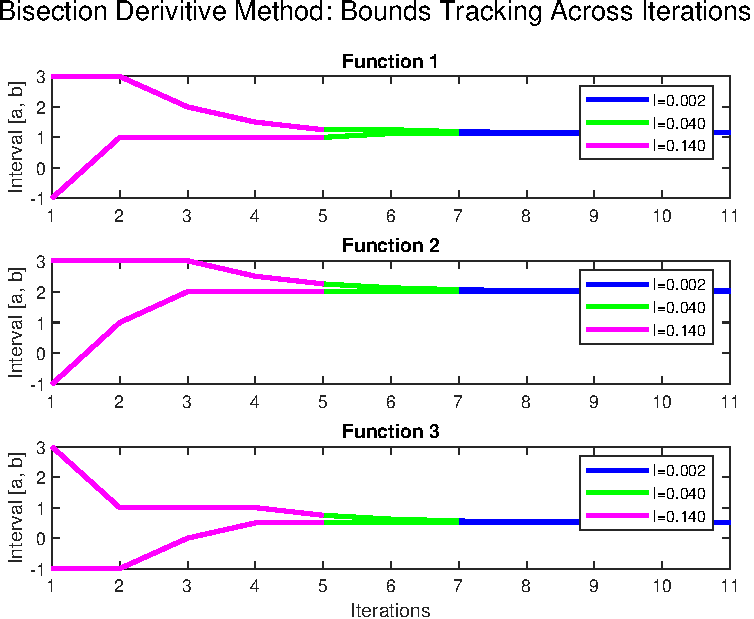
\includegraphics[width=0.75\linewidth]{plots/task4_plot2.pdf}
    \caption{Μεταβολή του διαστήματος $[\alpha_k, \beta_k]$ σε κάθε επανάληψη της μεθόδου διχοτόμησης με χρήση παραγώγου για διάφορες τιμές του $l$}
    \label{fig:task4_plot2}
\end{figure}

Τέλος, στο Σχήμα~\ref{fig:task0_plot1} φαίνονται ο αριθμός των υπολογισμών της αντικειμενικής συνάρτησης $f_1$ ή της
παραγώγου της για τις τέσσερις μεθόδους συναρτήσει του διαστήματος $l$. Παρατηρούμε ότι η πιο αποδοτική είναι η
μέθοδος της διχοτόμησης με χρήση παραγώγου, ακολουθεί η μέθοδος $fibonacci$ η οποία είναι ελαφρώς καλύτερη από
την μέθοδο του χρυσού τομέα ενώ η πιο υπολογιστικά κοστοβόρα είναι η μέθοδος διχοτόμησης. Επίσης στο 
Σχήμα~\ref{fig:task0_plot2} φαίνεται ο αριθμός των επαναλήψεων της κάθε μεθόδου συναρτήσει του $l$ για την $f_1$.
Βλέπουμε ότι η μέθοδος διχοτόμησης με χρήση παραγώγου απαιτεί τις λιγότερες επαναλήψεις, ακολουθεί η απλή 
μέθοδος διχοτόμησης η οποία απαιτεί ελαφρώς περισσότερες, έπειτα η μέθοδος $fibonacci$ και τέλος η μέθοδος του
χρυσού τομέα που απαιτεί ελαφρώς περισσότερες από την μέθοδο $fibonacci$.

\begin{figure}
    \centering
    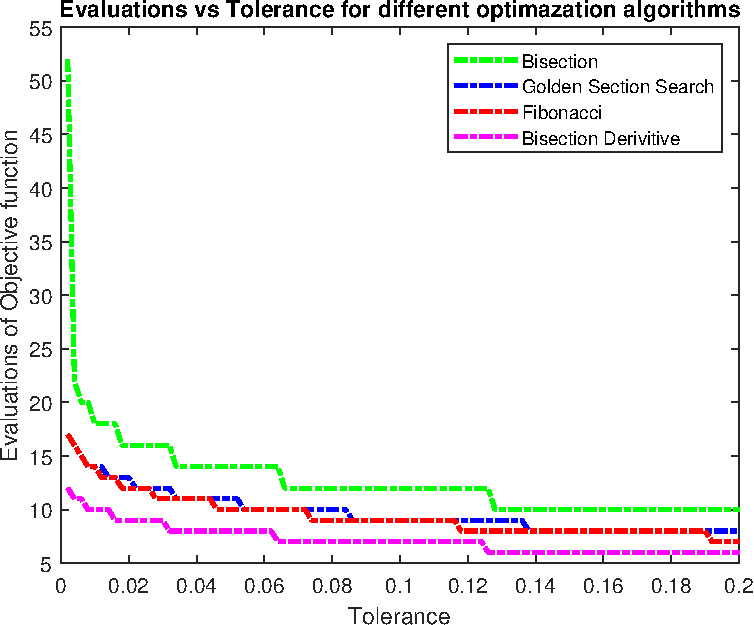
\includegraphics[width=0.75\linewidth]{plots/task0_plot1.pdf}
    \caption{Aριθμός των υπολογισμών της αντικειμενικής συνάρτησης $f_1$ συναρτήσει του $l$ για τις τέσσερις μεθόδους}
    \label{fig:task0_plot1}
\end{figure}

\begin{figure}
    \centering
    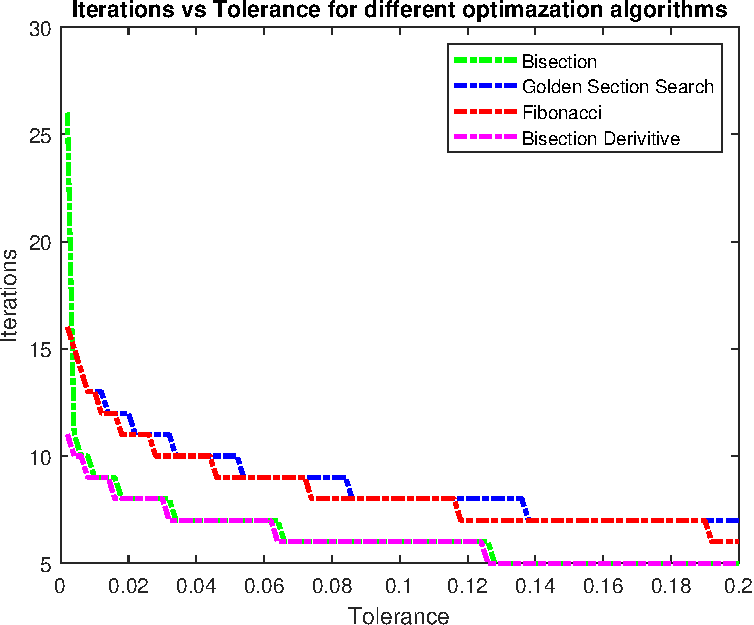
\includegraphics[width=0.75\linewidth]{plots/task0_plot2.pdf}
    \caption{Αριθμός επαναλήψεων των τεσσάρων μεθόδων συναρτήσει του $l$ για την αντικειμενική συνάρτηση $f_1$}
    \label{fig:task0_plot2}
\end{figure}

\section*{Συμπέρασμα}

Από την παραπάνω ανάλυση προκύπτει ότι μέθοδος της διχοτόμου με χρήση παραγώγου είναι η πιο αποδοτική τόσο
ως προς το πλήθος των υπολογισμών της αντικειμενικής συνάρτησης, όσο και ως προς τον αριθμό των επαναλήψεων
που απαιτούνται. Ωστόσο προϋποθέτει την γνώση της παραγώγου της υπό μελέτη συνάρτησης καθώς και τον εκ των
προτέρων υπολογισμό του πλήθους των επαναλήψεων για δεδομένη ακρίβεια. Από τις μεθόδους αναζήτησης ελαχίστου 
χωρίς την χρήση παραγώγων η πιο αποδοτική από άποψη υπολογιστικού κόστους είναι η μέθοδος $fibonacci$. Τέλος,
η μέθοδος της διχοτόμου, αν και απαιτεί μικρό αριθμό επαναλήψεων για να συγκλίνει στο επιθυμητό διάστημα,
είναι υπολογιστικά δαπανηρή καθιστώντας την ακατάλληλη για προβλήματα που απαιτούν μεγάλη ακρίβεια.

\end{document}
